\section{MHD Tests}
\label{sec:mhd-tests}

In this Section, we show the results of a suite of test problems that demonstrate the accuracy, robustness and performance of Cholla MHD. We have included many problems that are common in the literature and specifically selected tests that are challenging for the integrator and, when possible, have quantifiable measures of correctness for comparison to other methods and codes. All of these problems are also included in our automated test suite as either accuracy and/or regression system tests (see Section \ref{sec:testing} for details). Section \ref{sec:accuracy_tests} discusses tests for accuracy, while Section \ref{sec:mhd-perf-tests} discusses the performance and scaling of Cholla MHD.

\subsection{Accuracy Tests}
\label{sec:accuracy_tests}

\subsubsection{Linear Wave Convergence}
\label{sec:lwc}

The propagation of the four MHD linear waves provides an excellent quantitative measure of the accuracy of a numberical MHD method. Our linear wave tests use a periodic domain of $1.0\times1.0\times1.0$ and a resolution of $N\times16\times16$ where $N$ goes from 16 to 512 in powers of 2. The wave equation is

\begin{equation}
    q = \overline{q} + A R_w \sin{\frac{2\pi x}{\lambda}},
\end{equation}

\noindent where $q$ is the conserved variable, $\overline{q}$ is the mean background state, $A=10^{-6}$ is the amplitude of the wave, $R_w$ is the right eigenvector in conserved variables for the wave mode $w$, $x$ is the position, and $\lambda=1$ is the wavelength of the wave. The adiabatic index $\gamma$ is $5/3$ and the background state is:
$\overline{\rho}=1.0$,
$\overline{v_x}=\overline{v_y}=\overline{v_z}=0$ (except for the contact wave where $\overline{v_x} = 1$),
$\overline{P}=1/\gamma$,
$\overline{B_x}=1$,
$\overline{B_y}=1.5$,
and $\overline{B_z}=0$.
The right eigenvectors for this state are given in Appendix A of \cite{gardiner_unsplit_2008}.

The wave propagates for one period, after which the error is computed between the initial and final state. First we compute the L1 norm, which is the absolute difference for each conserved variable between the initial and final state:

\begin{equation}
    \delta q_s = \frac{1}{n_x n_y n_z} \sum_{i,j,k} \mid q^f_{i,j,k,s} - q^i_{i,j,k,s} \mid,
\end{equation}

\noindent where $q_s$ is a specific conserved variable. We then compute the L2 norm of this vector of L1 norms as

\begin{equation}
    \mid \mid \delta q \mid \mid = \sqrt{\sum_s \left( \delta q_s \right)^2}.
\end{equation}

These L2 errors are plotted in \autoref{fig:linear-wave-convergence} for both the PLM and PPM reconstructions. The results are comparable to the results in \cite{stone_2009} and demonstrate the expected second order convergence. Using PPM improves the accuracy of the solution by approximately an order of magnitude at any given resolution, but maintains the second order convergence due to the second order nature of the integrator. We have implemented these tests in all three directions with the waves moving in the positive or negative directions and find identical results.

\begin{figure}[ht!]
    % \epsscale{0.5}
    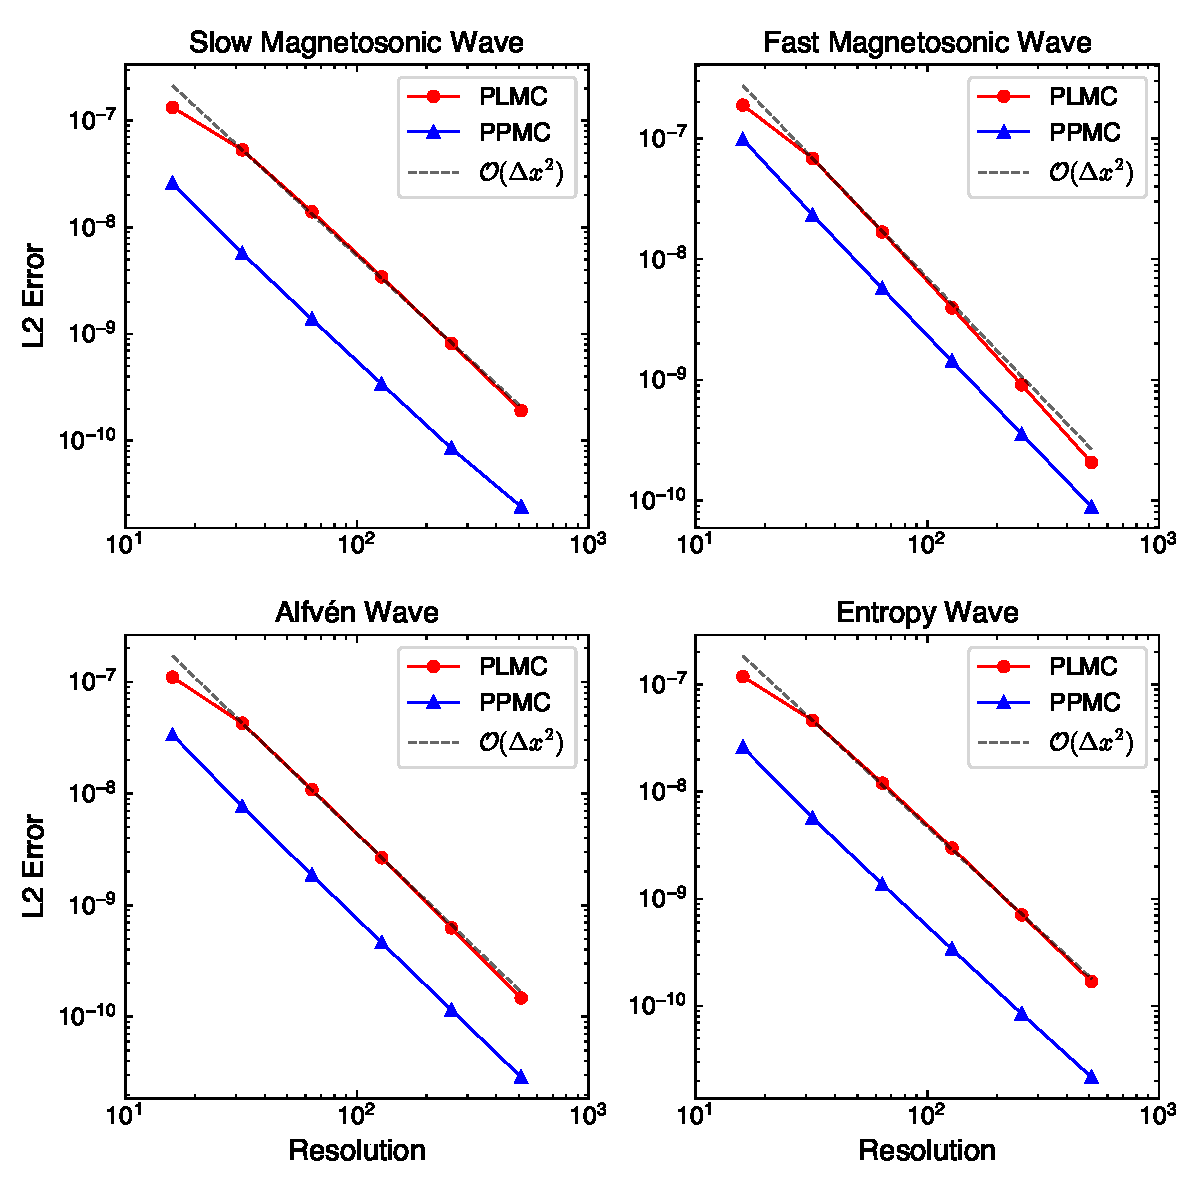
\includegraphics[width=\linewidth]{linear_convergence.pdf}
    \caption{Linear Wave Convergence of all four MHD waves using PLM and PPM reconstruction. \href{https://github.com/bcaddy/caddy-et-al-2023/blob/a5d284c28192e6ae8b0c09e82f75a36456cf0ca6/python/linear-wave-convergence.py}{\img{../latex-src/github.png}}}
    \label{fig:linear-wave-convergence}
\end{figure}

\subsubsection{Circularly Polarized Alfv\'en Wave}
\label{sec:cpaw}

The circularly polarized Alfv\'en wave is a non-linear wave that tests a code's accuracy in the non-linear regime with the quantitative benefits of a regular wave test \citep{Toth1996}. The tests use a periodic domain of $3.0\times1.5\times1.5$ and a resolution of $2N\times N \times N$ where $N$ goes from 8 to 256 in powers of 2. The wave is initialized at an oblique angle the grid, making this a fully 3D test.

In a coordinate system aligned with the movement of the wave, the initial conditions are
$\rho = 1.0$,
$P = 0.1$,
$v_x = (0,-1)$ for traveling or standing waves respectively,
$v_y = A \sin{\frac{2\pi x}{\lambda}}$,
$v_z = A \cos{\frac{2\pi x}{\lambda}}$,
$B_x = 1.0$,
$B_y = A \sin{\frac{2\pi x}{\lambda}}$,
and $B_z = A \cos{\frac{2\pi x}{\lambda}}$,
where the amplitude of the wave $A = 0.1$ and the wavelength $\lambda = 1.0$. These coordinates are then transformed with the rotation

\begin{eqnarray}
    x\prime = x \cos\alpha\cos\beta - y \sin\beta - z \sin\alpha\cos\beta \nonumber \\
    y\prime = x \cos\alpha\sin\beta + y \cos\beta - z \sin\alpha\sin\beta \nonumber \\
    z\prime = x \sin\alpha + z \cos\alpha \nonumber
\end{eqnarray}

\noindent with $\sin\alpha = 2/3$ and $\sin\beta = 1/\sqrt{5}$. This ensures the domain is fully periodic through the boundaries and the wave can travel (or stand) indefinitely. The magnetic fields are initialized with the vector potential to ensure initial divergence is zero to round off. The waves are then run for a single period and the L2 norm of the L1 error vector is plotted in Figure \ref{fig:cpaw} using the same method as in Section \ref{sec:lwc}. It is interesting to note that the accuracy improvement of PPM versus PLM seen for the linear waves is absent in this non-linear test.

These Alfv\'en waves are subject to a parametric instability \citep{del_zanna_parametric_2001}, which should not be present for these initial conditions. However, the truncation error will result in small variations in the magnetic pressure which drives low amplitude compression waves \citep{stone_athena_2008}.

\begin{figure}[ht!]
    % \epsscale{0.5}
    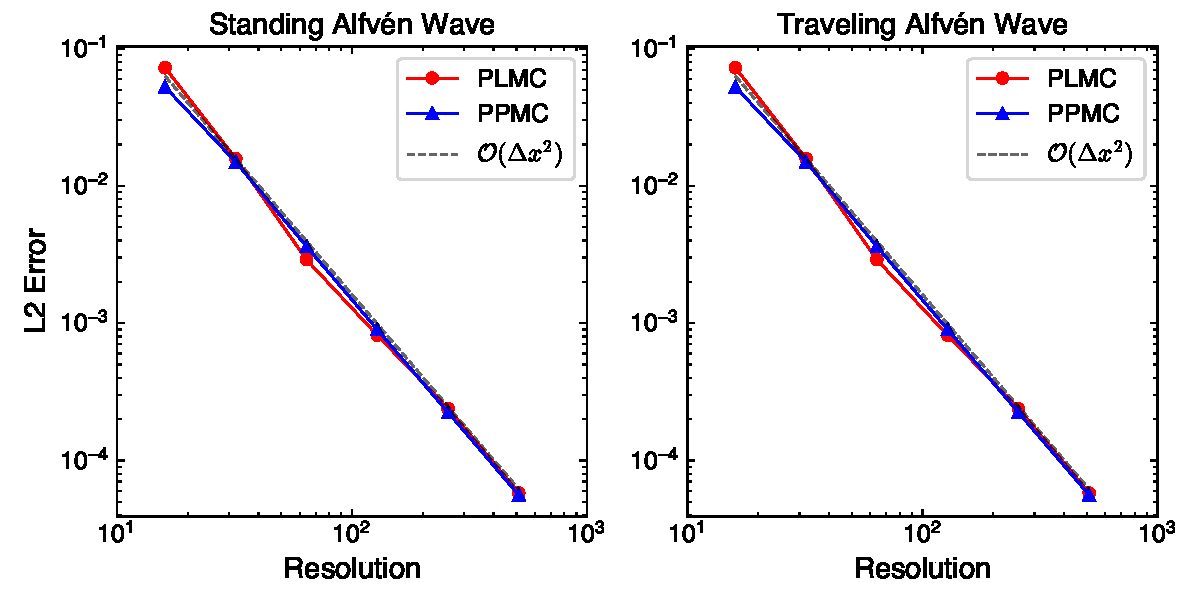
\includegraphics[width=\linewidth]{cpaw_convergence.pdf}
    \caption{Circularly Polarized Alfv\'en Wave Convergence using PLM and PPM reconstruction. \href{https://github.com/bcaddy/caddy-et-al-2023/blob/a5d284c28192e6ae8b0c09e82f75a36456cf0ca6/python/circularly-polarized-alfven-convergence.py}{\img{../latex-src/github.png}}}
    \label{fig:cpaw}
\end{figure}

\subsubsection{Advecting Field Loop}
\label{sec:afl}

The advecting field loop test consists of a tilted spherical current loop which travels across the domain at an oblique angle to the grid. This test requires particularly accurate balancing of the non-zero components of the induction equation. It also has zero magnetic field outside the spherical current loop; as the current loops moves across the grid those cells that are no longer in the loop should return to zero to within round off error. It is also a good test of the dissipation of the magnetic field, as the magnetic pressure should remain constant.

The initial conditions for this test are most easily described using the magnetic vector potential, which is the vector quantity whose curl equals the magnetic field, $\boldsymbol{B} = \nabla \times\boldsymbol{A}$. The background state is
$\rho = 1.0$,
$P = 1.0$,
$v_x = 1.0$,
$v_y = 1.0$,
$v_z = 2.0$,
$B_x = 0$,
$B_y = 0$, and
$B_z = 0$.

In the central region the state is given by the following vector potential, which we have chosen such that $A_x = 0$:
\begin{equation}
    A_y = A_z =
    \begin{cases}
        A \left( R - r \right),& \text{for}\; r < R\\
        0,              & \text{otherwise}
    \end{cases}
\end{equation}

\noindent where $r$ is the Euclidean distance from the center of the domain. Note that since the vector potential is along the vertices of the cells, $A_y$ and $A_z$ will never have the same value at the same position as they are not stored at identical positions. The test is conducted on a grid of $N\times N\times 2N$ cells for $N=(32, 64, 128, 256)$ with a periodic domain of $1.0\times1.0\times2.0$ centered at zero and evolved for two periods; $t_{max} = 2.0$.

Figure \ref{fig:afl} shows the mean of cell centered $B^2$, normalized to the initial value, in order to demonstrate the convergence of the dissipation rate. The dissipation rate is comparable to those found in the literature \citep{stone_athena_2008} and improves at approximately first order. Figure \ref{fig:afl} also shows the maximum divergence in the domain as a function of time. Throughout the entire evolution it remains near round off and, after an initial rise, remains fairly constant. The zero magnetic field region outside of the current loop also remains near zero throughout the entire evolution of the problem.

\begin{figure}[ht!]
    % \epsscale{0.5}
    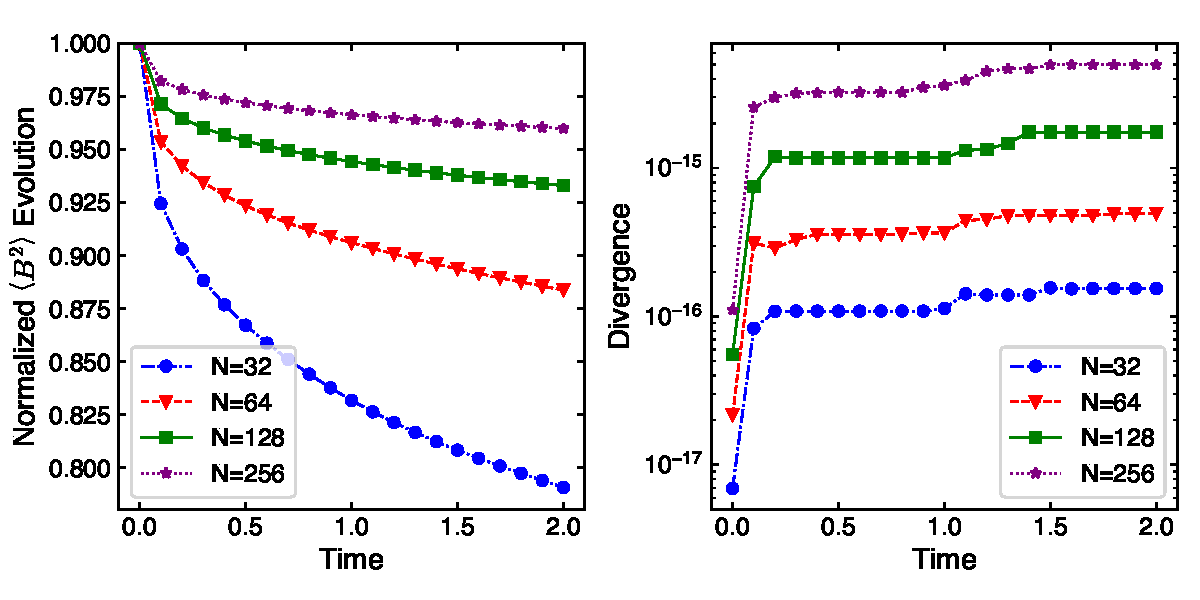
\includegraphics[width=\linewidth]{afl.pdf}
    \caption{Evolution of tilted spherical magnetic field loop through two full periods. Mean of $B^2$ normalized to the initial value as a function of time (left) and the maximum divergence in the domain as a function of time (right). \href{https://github.com/bcaddy/caddy-et-al-2023/blob/a5d284c28192e6ae8b0c09e82f75a36456cf0ca6/python/advecting-field-loop.py}{\img{../latex-src/github.png}}}
    \label{fig:afl}
\end{figure}

\subsubsection{MHD Riemann Problems}
\label{sec:riemann}

MHD Riemann problems are standard tests for new MHD codes and methods due to their mix of different flow types and extreme conditions. There are many different MHD Riemann problems in the literature \citep{brio_wu_1988, einfeldt_1991, ryu_jones_1995, dai_woodward_1998}; we have chosen to present five that cover a variety of challenging cases.

The Riemann problem is defined as having a single state for half of the domain which suddenly switches at a discontinuity to a different state on the other half of the domain. All of Riemann problems here have a domain of $1\times1\times1$ and resolution of $512\times16\times16$ and are run until the $t_{max}$ for that particular Riemann problem and utilize parabolic reconstruction with limiting in the characteristic variables. All have been run in all three spatial directions with both possible orientations of the two states and achieved identical results. The details of each left and right state are given in Table \ref{table:riemann}.

% Can add a * after "deluxetable" in begin and end to let it span 2 columns

%% The values (usually only l,r and c) in the last part of
%% \begin{deluxetable}{} command tell LaTeX how many columns
%% there are and how to align them.
\begin{deluxetable*}{lccccccccccccccccc}
    \label{table:riemann}
    
    %% Over-ride the default font size
    %% Use Default (12pt)
    
    %% Use \tablewidth{?pt} to over-ride the default table width.
    %% If you are unhappy with the default look at the end of the
    %% *.log file to see what the default was set at before adjusting
    %% this value.
    
    %% This is the title of the table.
    \tablecaption{Riemann Problem Initial Conditions}
    
    %% The \tablehead gives provides the column headers.  It
    %% is currently set up so that the column labels are on the
    %% top line and the units surrounded by ()s are in the 
    %% bottom line.  You may add more header information by writing
    %% another line between these lines. For each column that requries
    %% extra information be sure to include a \colhead{text} command
    %% and remember to end any extra lines with \\ and include the 
    %% correct number of &s.
    \tablehead{\colhead{Riemann Problem} & \colhead{$\gamma$} & \colhead{$t_{max}$} & \colhead{$B_x$} & 
    \colhead{$\rho_L$} & \colhead{$P_L$} & \colhead{$v_{x,L}$} & \colhead{$v_{y,L}$} & \colhead{$v_{z,L}$} & \colhead{$B_{y,L}$} & \colhead{$B_{z,L}$} & 
    \colhead{$\rho_R$} & \colhead{$P_R$} & \colhead{$v_{x,R}$} & \colhead{$v_{y,R}$} & \colhead{$v_{z,R}$} & \colhead{$B_{y,R}$} & \colhead{$B_{z,R}$}}
    
    %% All data must appear between the \startdata and \enddata commands
    \startdata
    % Riemann Problem      gamma           t_max  B_x                       rho_L  P_L    V_x,L  V_y,L  V_z,L B_y,L                       B_z,L                     rho_R   P_R    V_x,R   V_y,R V_z,R B_y,R                     B_z,R
    Brio \& Wu           & 2             & 0.1  & 0.75                    & 1    & 1    & 0    & 0    & 0   & 1                         & 0                       & 0.128 & 0.1  & 0     & 0   & 0   & -1                      & 0                       \\
    Dai \& Woodward      & $\frac{5}{3}$ & 0.2  & $\frac{2}{\sqrt{4\pi}}$ & 1.08 & 0.95 & 1.2  & 0.01 & 0.5 & $\frac{3.6}{\sqrt{4\pi}}$ & $\frac{2}{\sqrt{4\pi}}$ & 1     & 1    & 0     & 0   & 0   & $\frac{4}{\sqrt{4\pi}}$ & $\frac{2}{\sqrt{4\pi}}$ \\
    Ryu \& Jones 1a      & $\frac{5}{3}$ & 0.08 & $\frac{5}{\sqrt{4\pi}}$ & 1    & 20   & 10   & 0    & 0   & $\frac{5}{\sqrt{4\pi}}$   & 0                       & 1     & 1    & -10   & 0   & 0   & $\frac{5}{\sqrt{4\pi}}$ & 0                       \\
    Ryu \& Jones 4d      & $\frac{5}{3}$ & 0.16 & 0.7                     & 1    & 1    & 0    & 0    & 0   & 0                         & 0                       & 0.3   & 0.2  & 0     & 0   & 1   & 1                       & 0                       \\
    Einfeldt Rarefaction & 1.4           & 0.16 & 0                       & 1    & 0.45 & -2   & 0    & 0   & 0.5                       & 0                       & 1     & 0.45 & 2     & 0   & 0   & 0.5                     & 0                       \\
    \enddata
    
    %% Include any \tablenotetext{key}{text}, \tablerefs{ref list},
    %% or \tablecomments{text} between the \enddata and 
    %% \end{deluxetable} commands
    
    %% General table comment marker
    \tablecomments{The $L/R$ subscripts indicate that it is the left/right state. $B_x$ is always the same in both states.}
    
\end{deluxetable*}

\paragraph{Brio \& Wu Shock Tube}

The Brio \& Wu Shock Tube \citep{brio_wu_1988} is a staple test of MHD codes. This Riemann problem is essentially the Sod shock tube \citep{sod_1978} with a magnetic field. However, this shock tube is an excellent stress test for PPM reconstruction, as methods higher than second order tend to create large oscillations in the solution due to the slowly moving shock waves. We have implemented both the PPM reconstruction algorithm used in the VL+CT integrator from the method described in \cite{stone_athena_2008} as well as the method described in \cite{felker_2018}, and find that the latter significantly reduces oscillations for this test. With PPM reconstruction, we find  oscillations in the solution when limiting in either the primitive or characteristic variables. No oscillations are present when using PLM reconstruction.

\begin{figure}[ht!]
    % \epsscale{0.5}
    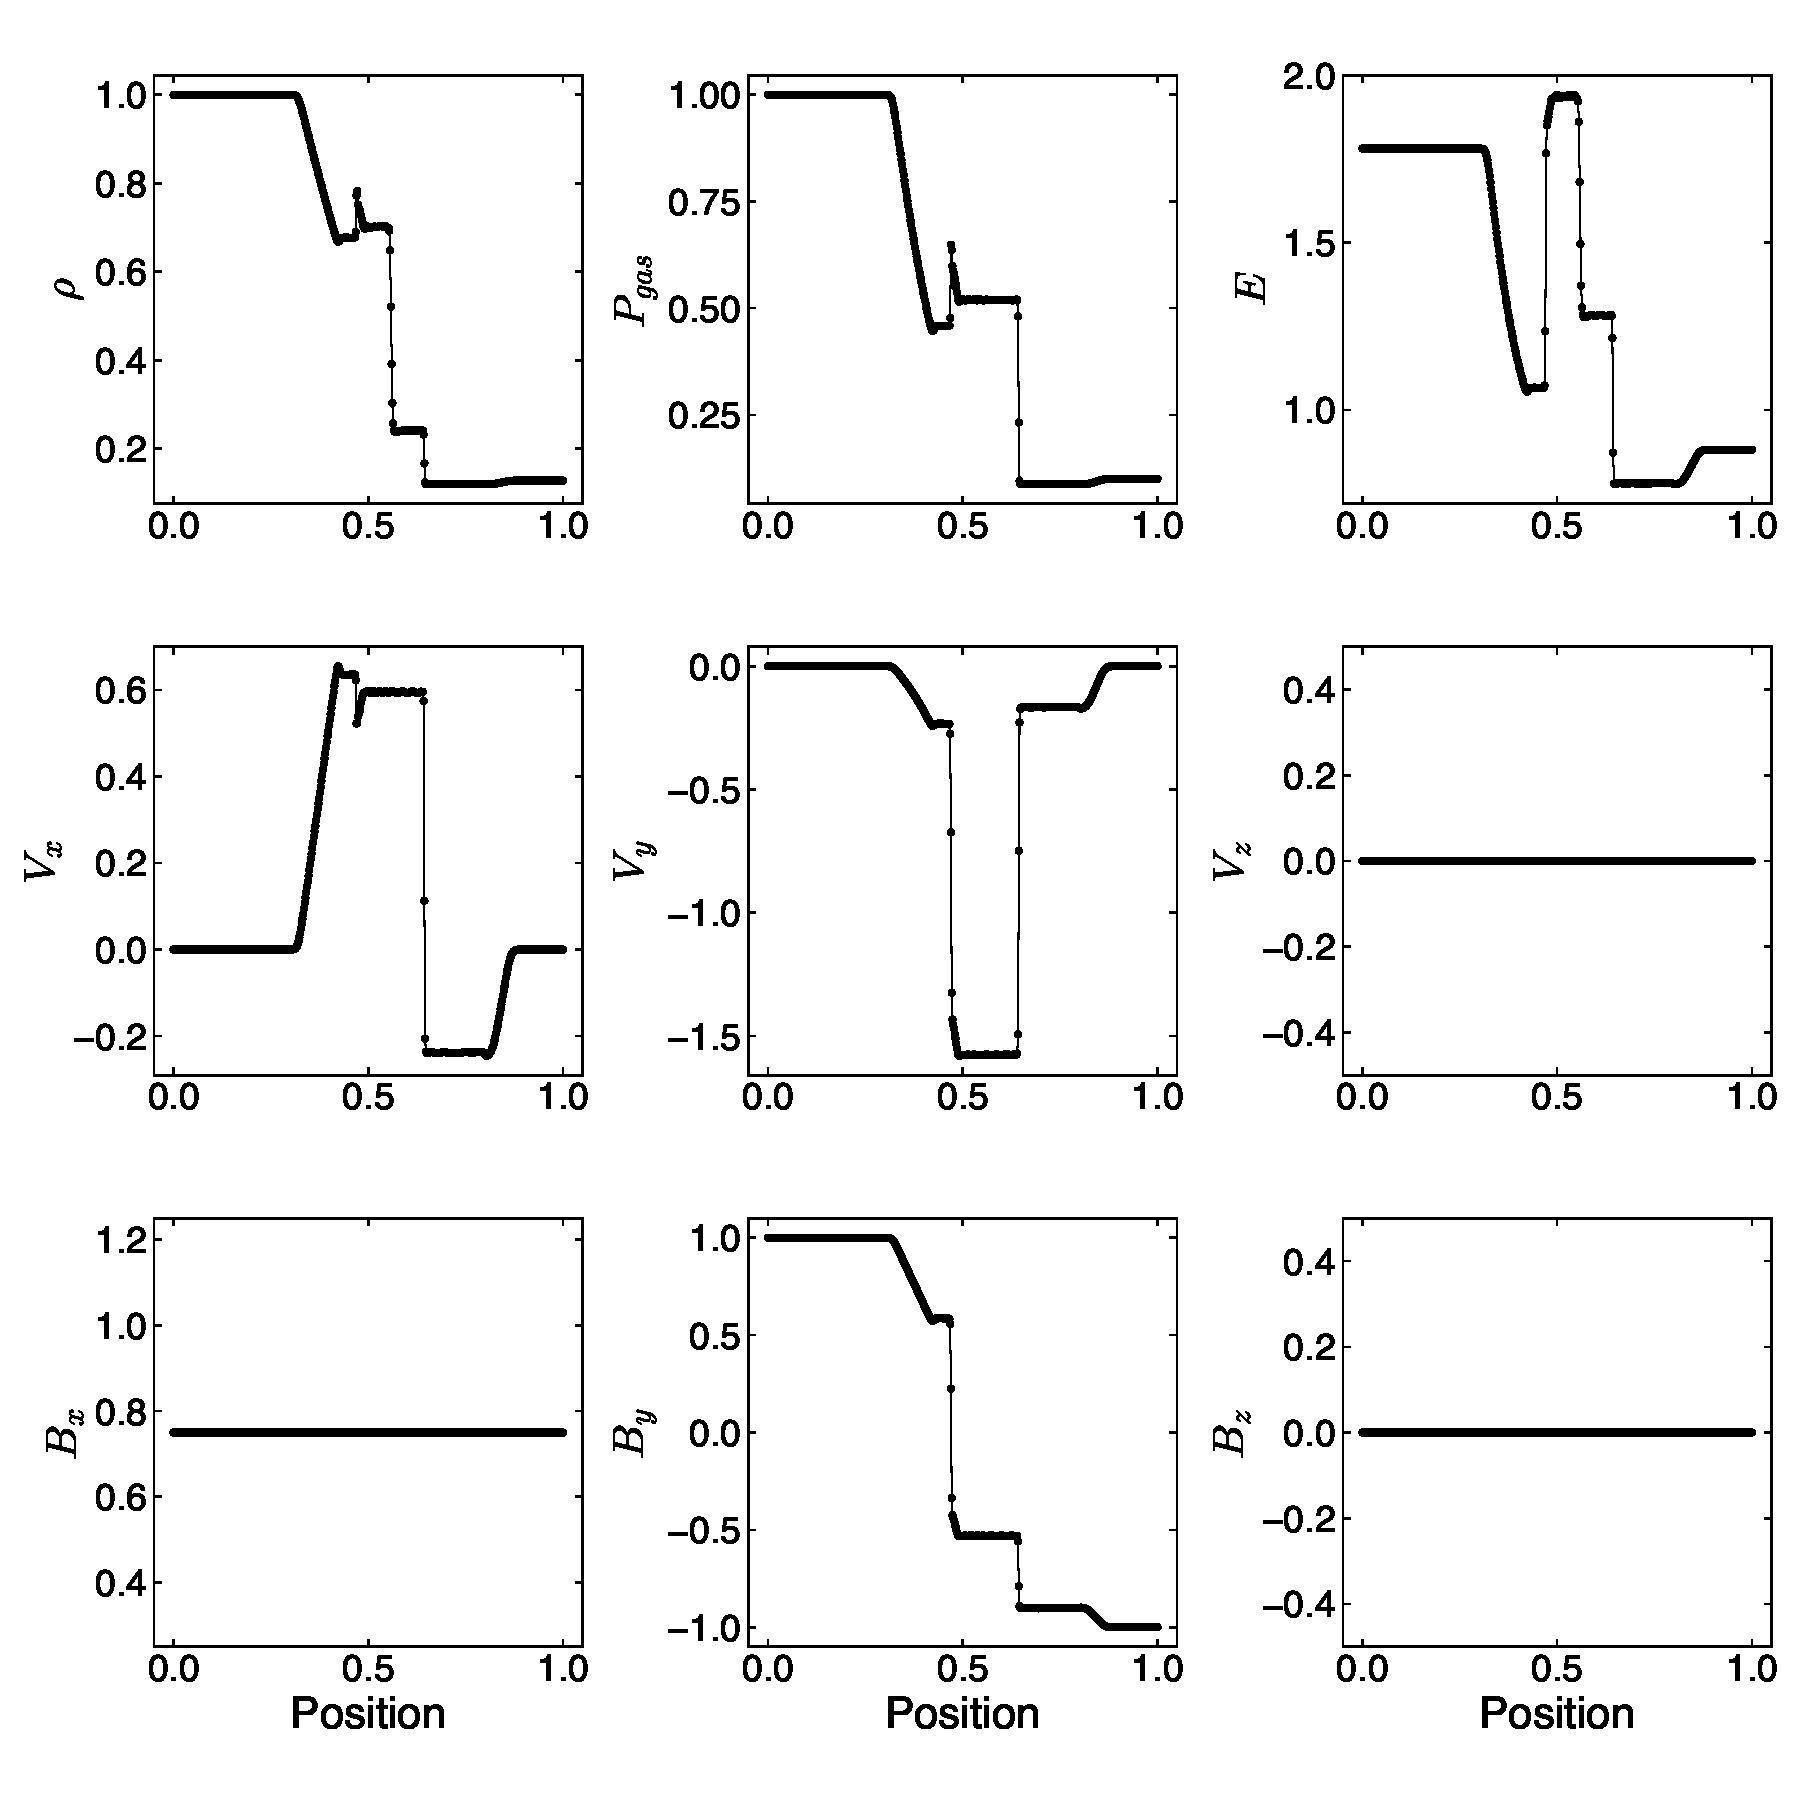
\includegraphics[width=\linewidth]{b&w.pdf}
    \caption{The Brio \& Wu Shock Tube solution \citep{brio_wu_1988}.
    \href{https://github.com/bcaddy/caddy-et-al-2023/blob/4c9c5ef905902e54e50943d0a261bd5b08342225/python/shock-tubes.py}{\img{../latex-src/github.png}}}
    \label{fig:brio-and-wu}
\end{figure}

\paragraph{Dai \& Woodward Shock Tube}

The Dai \& Woodward Shock Tube (also called Ryu \& Jones 2a) \citep{dai_woodward_1998, ryu_jones_1995} produces all seven possible MHD waves. From left to right they are: fast shock, Alfvén wave, slow shock, contact discontinuity, slow shock, Alfvén wave, and fast shock. This makes it an excellent laboratory for checking that the full spread of wave modes are well resolved.

\begin{figure}[ht!]
    % \epsscale{0.5}
    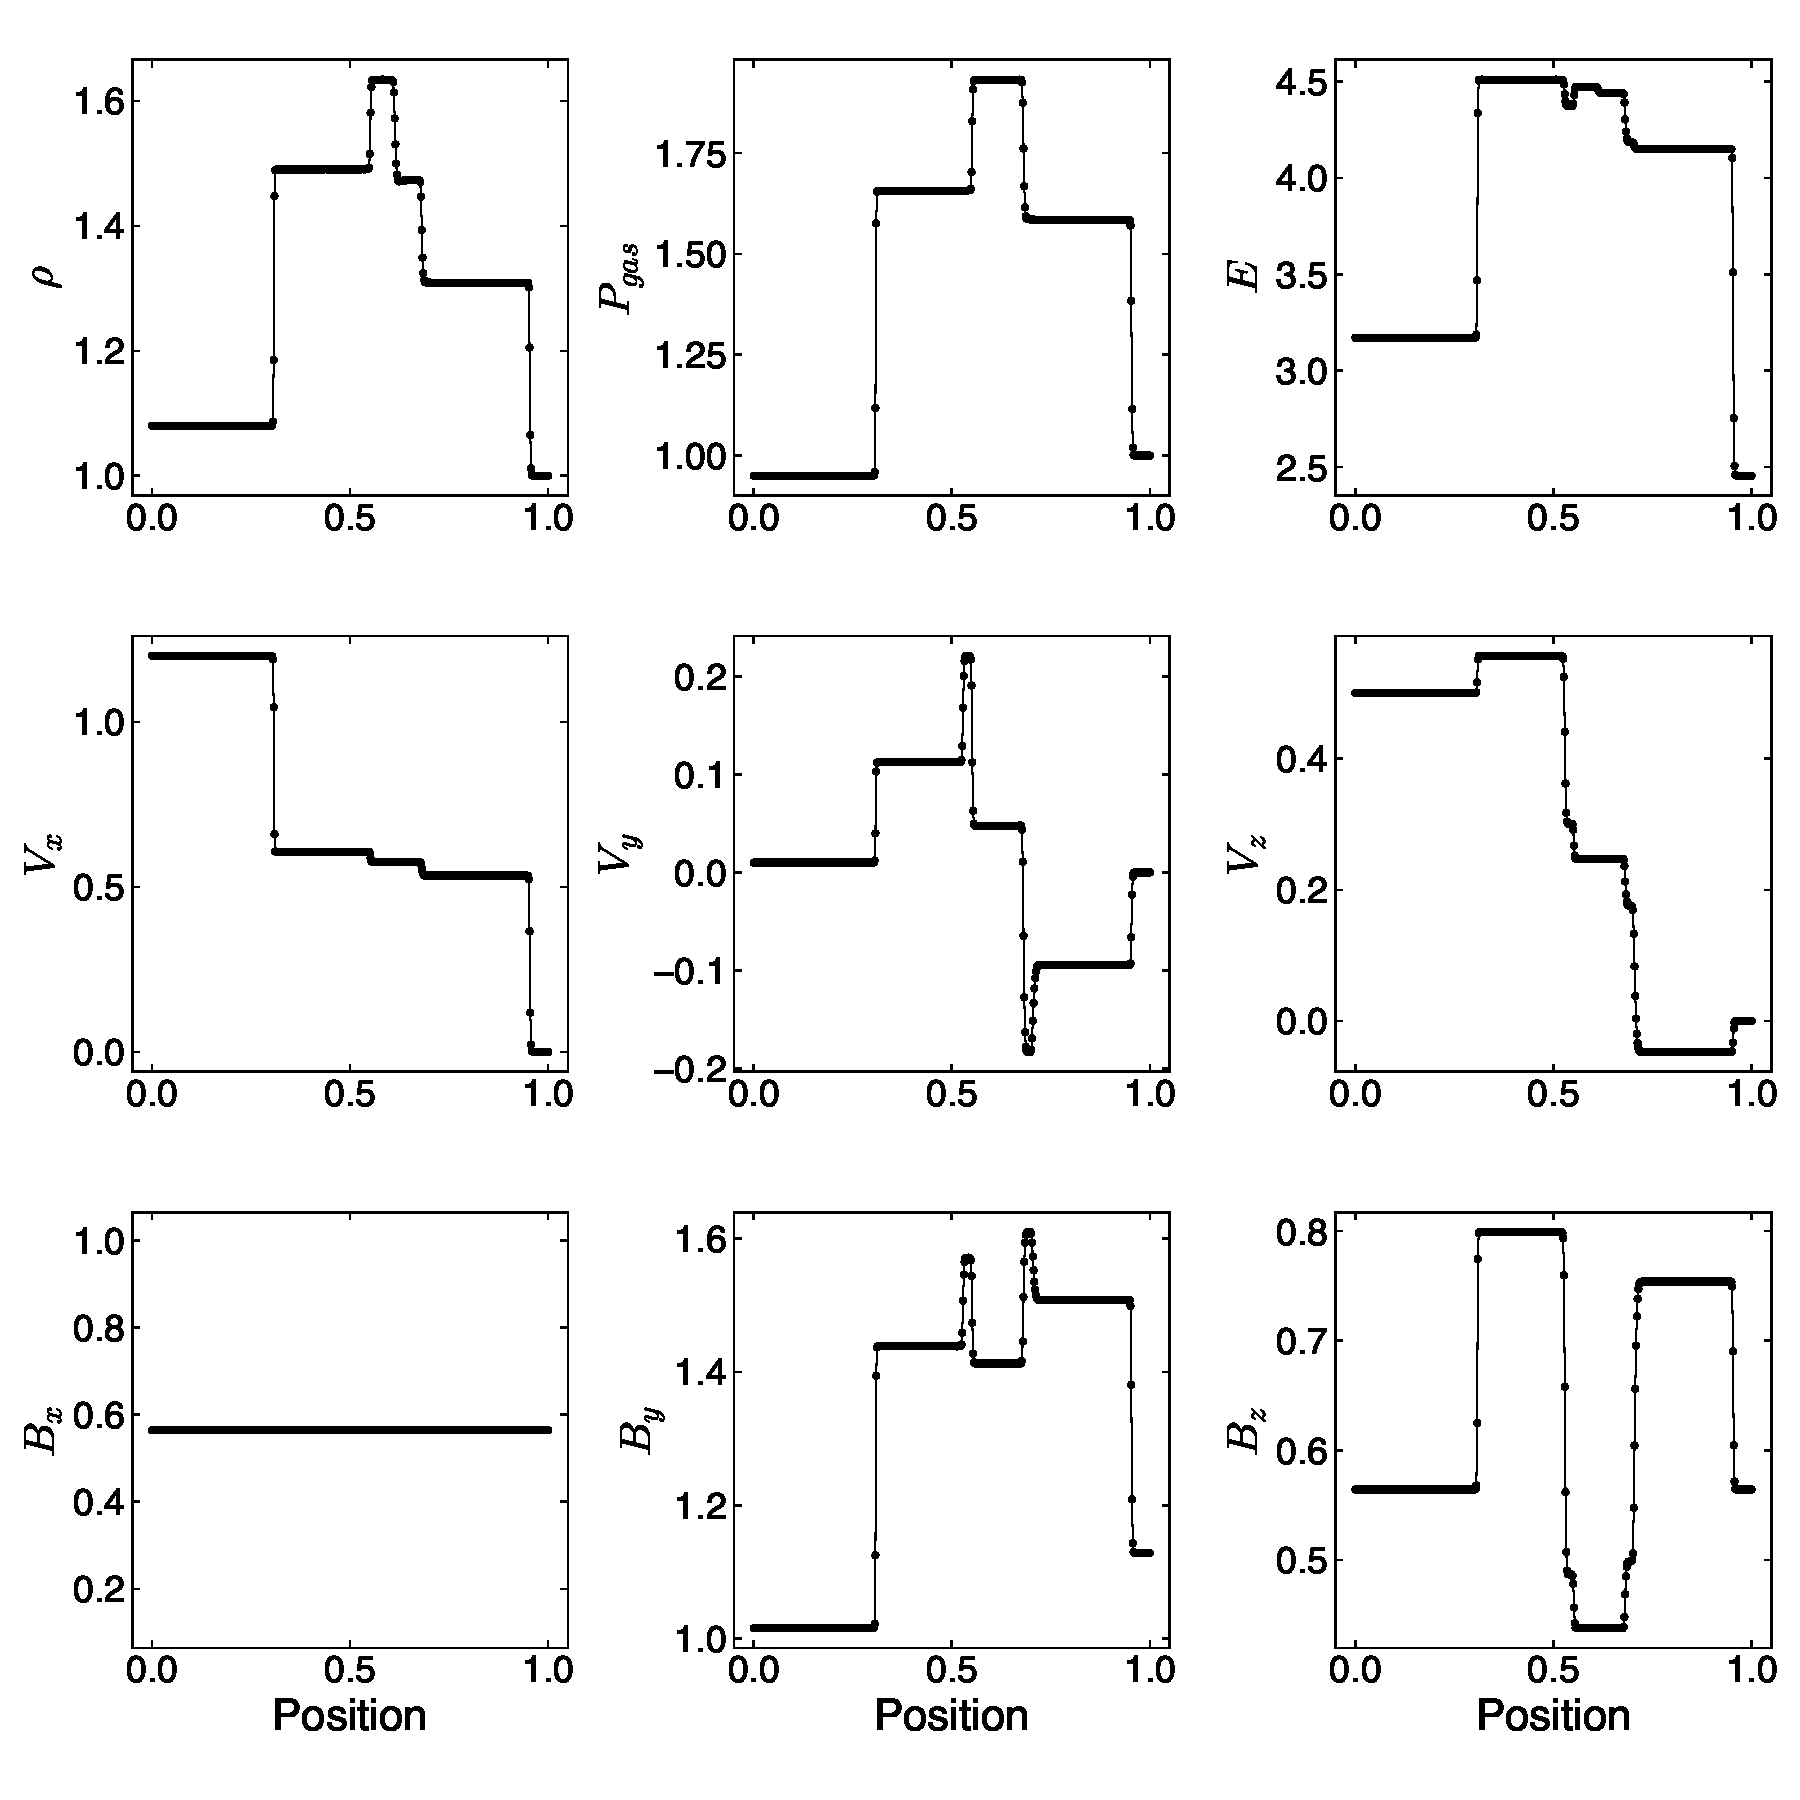
\includegraphics[width=\linewidth]{d&w.pdf}
    \caption{Dai \& Woodward Shock Tube (also called Ryu \& Jones 2a) solution \citep{dai_woodward_1998, ryu_jones_1995}.
    \href{https://github.com/bcaddy/caddy-et-al-2023/blob/4c9c5ef905902e54e50943d0a261bd5b08342225/python/shock-tubes.py}{\img{../latex-src/github.png}}}
    \label{fig:dai-and-woodward}
\end{figure}

\paragraph{Ryu \& Jones 1a Shock Tube}

Ryu \& Jones 1a Shock Tube solution \citep{ryu_jones_1995} is a less common test for MHD codes. However, in our experience, it is an excellent problem for debugging due to its relatively simple structure, which is easy to examine manually. The lack of any spikes and the presence of multiple types of strong shocks also make it a good diagnostic test for over/undershoot of the solution near discontinuities.

\begin{figure}[ht!]
    % \epsscale{0.5}
    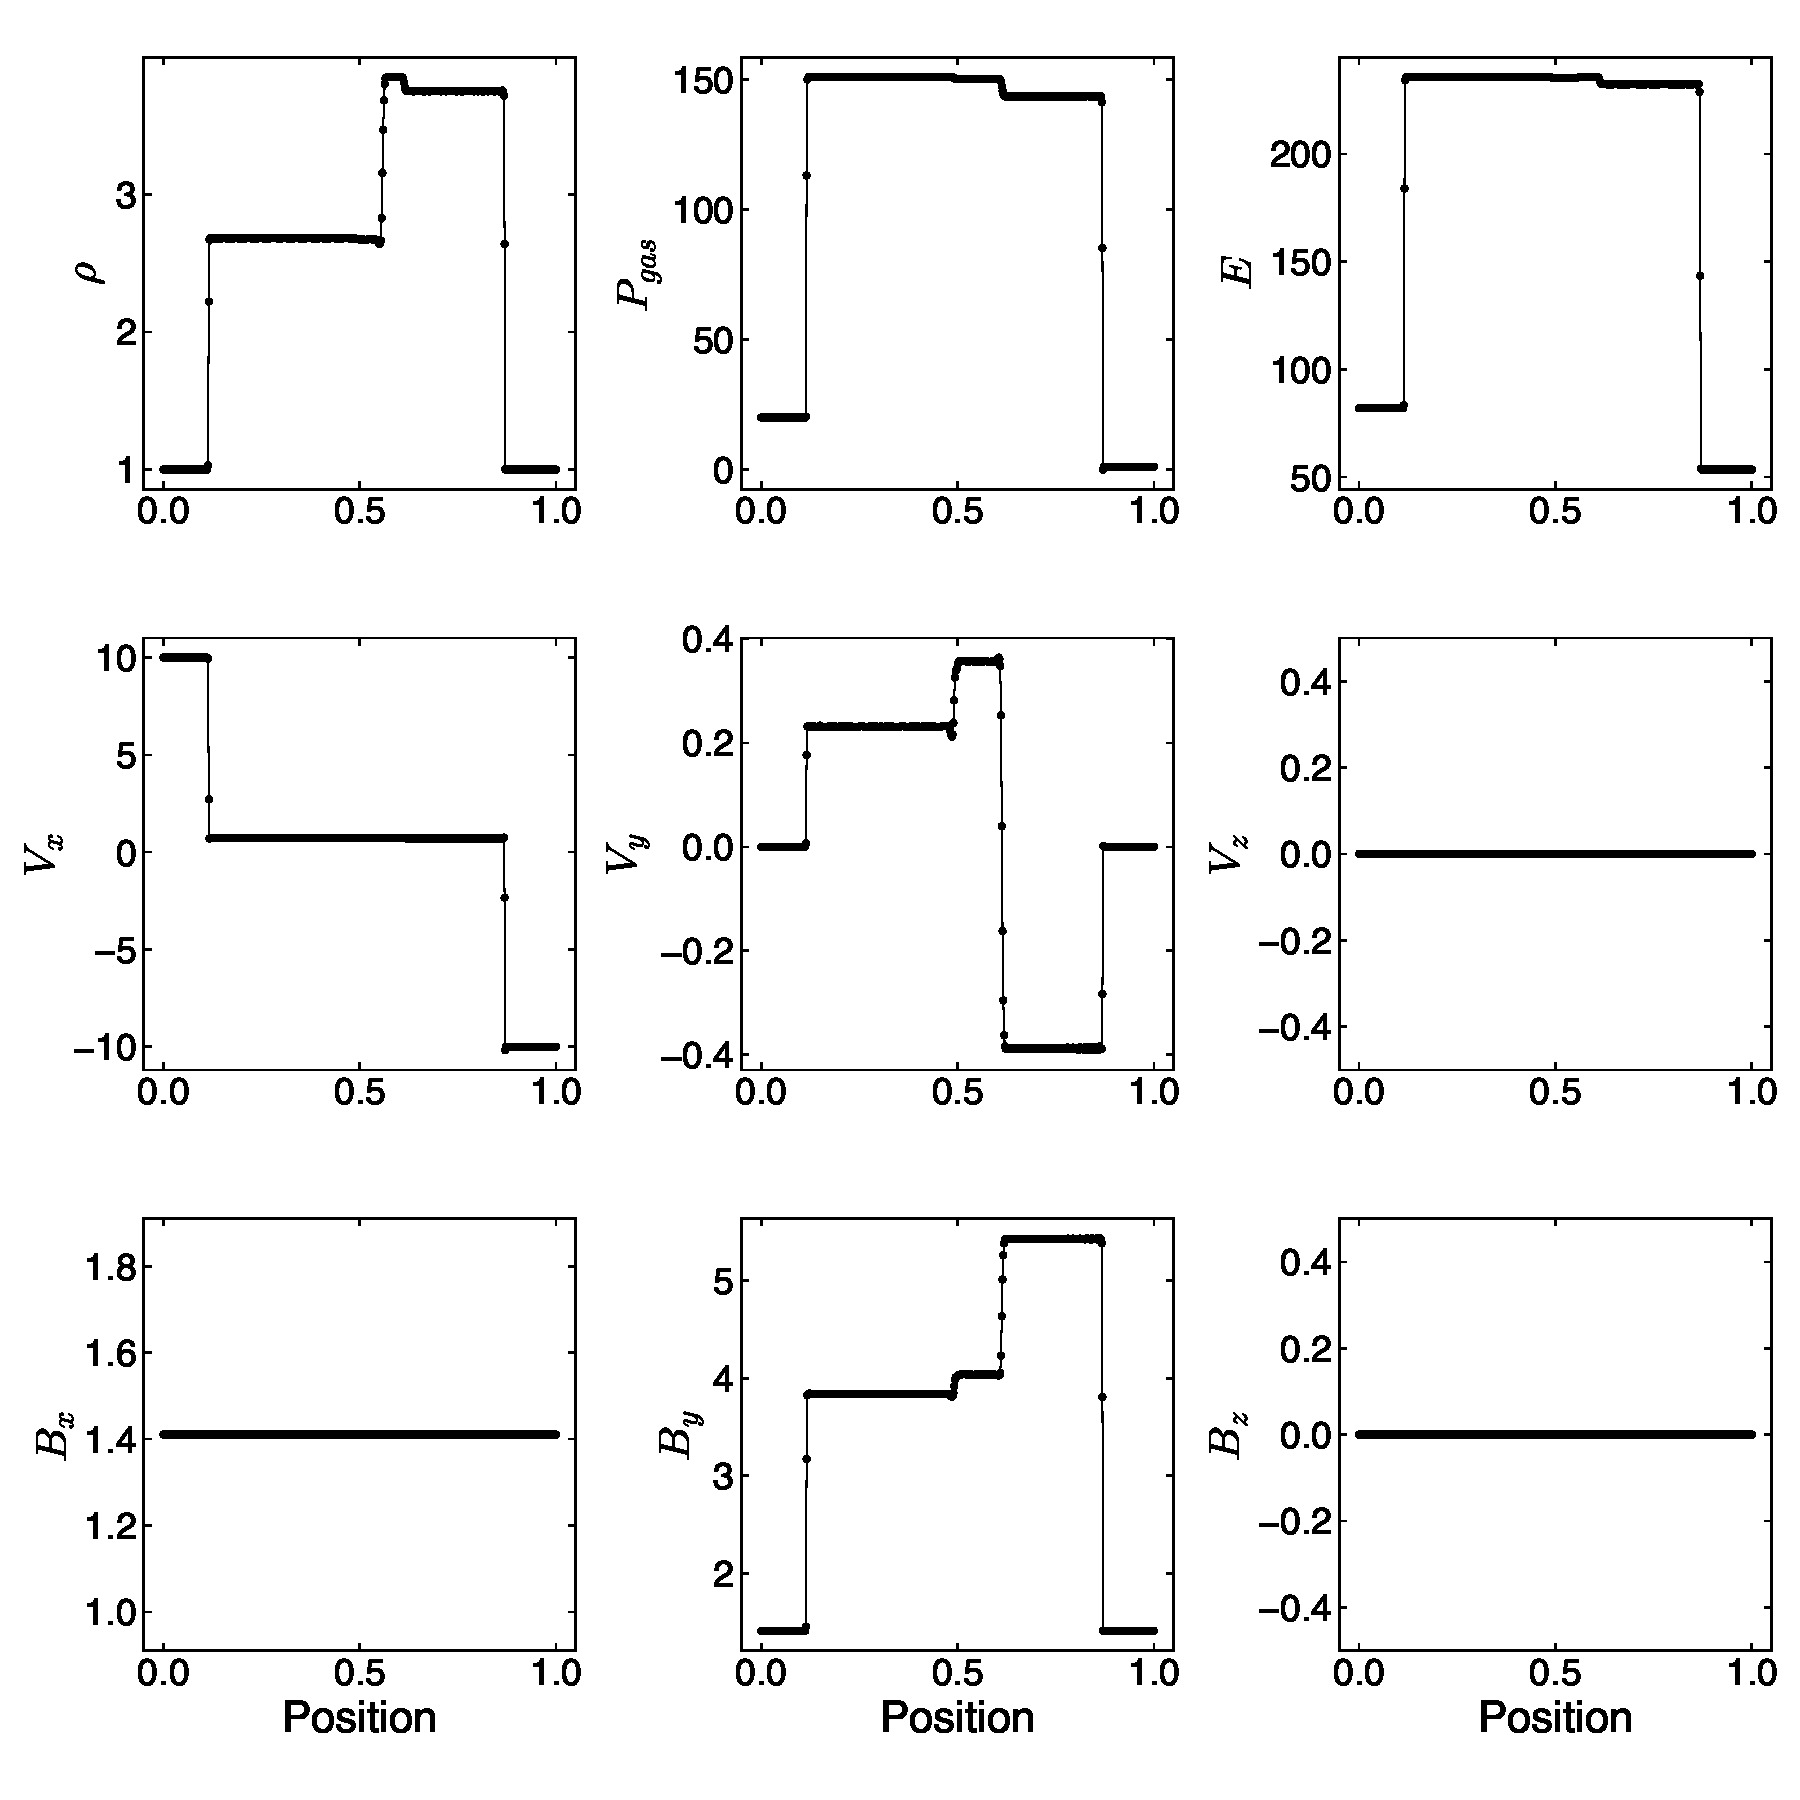
\includegraphics[width=\linewidth]{rj1a.pdf}
    \caption{Ryu \& Jones 1a Shock Tube solution \citep{ryu_jones_1995}.
    \href{https://github.com/bcaddy/caddy-et-al-2023/blob/4c9c5ef905902e54e50943d0a261bd5b08342225/python/shock-tubes.py}{\img{../latex-src/github.png}}}
    \label{fig:rj-1a}
\end{figure}

\paragraph{Ryu \& Jones 4d Shock Tube}

The Ryu \& Jones 4d Shock Tube solution \citep{ryu_jones_1995} features a switch-on slow shock. Switch-on waves increase the strength of the transverse magnetic field while reducing the thermal pressure to maintain energy conservation. This is a simplified example of a type of magnetic field amplification and as such it is important to demonstrate that a code can replicate it accurately. A switch-off wave does the inverse.

\begin{figure}[ht!]
    % \epsscale{0.5}
    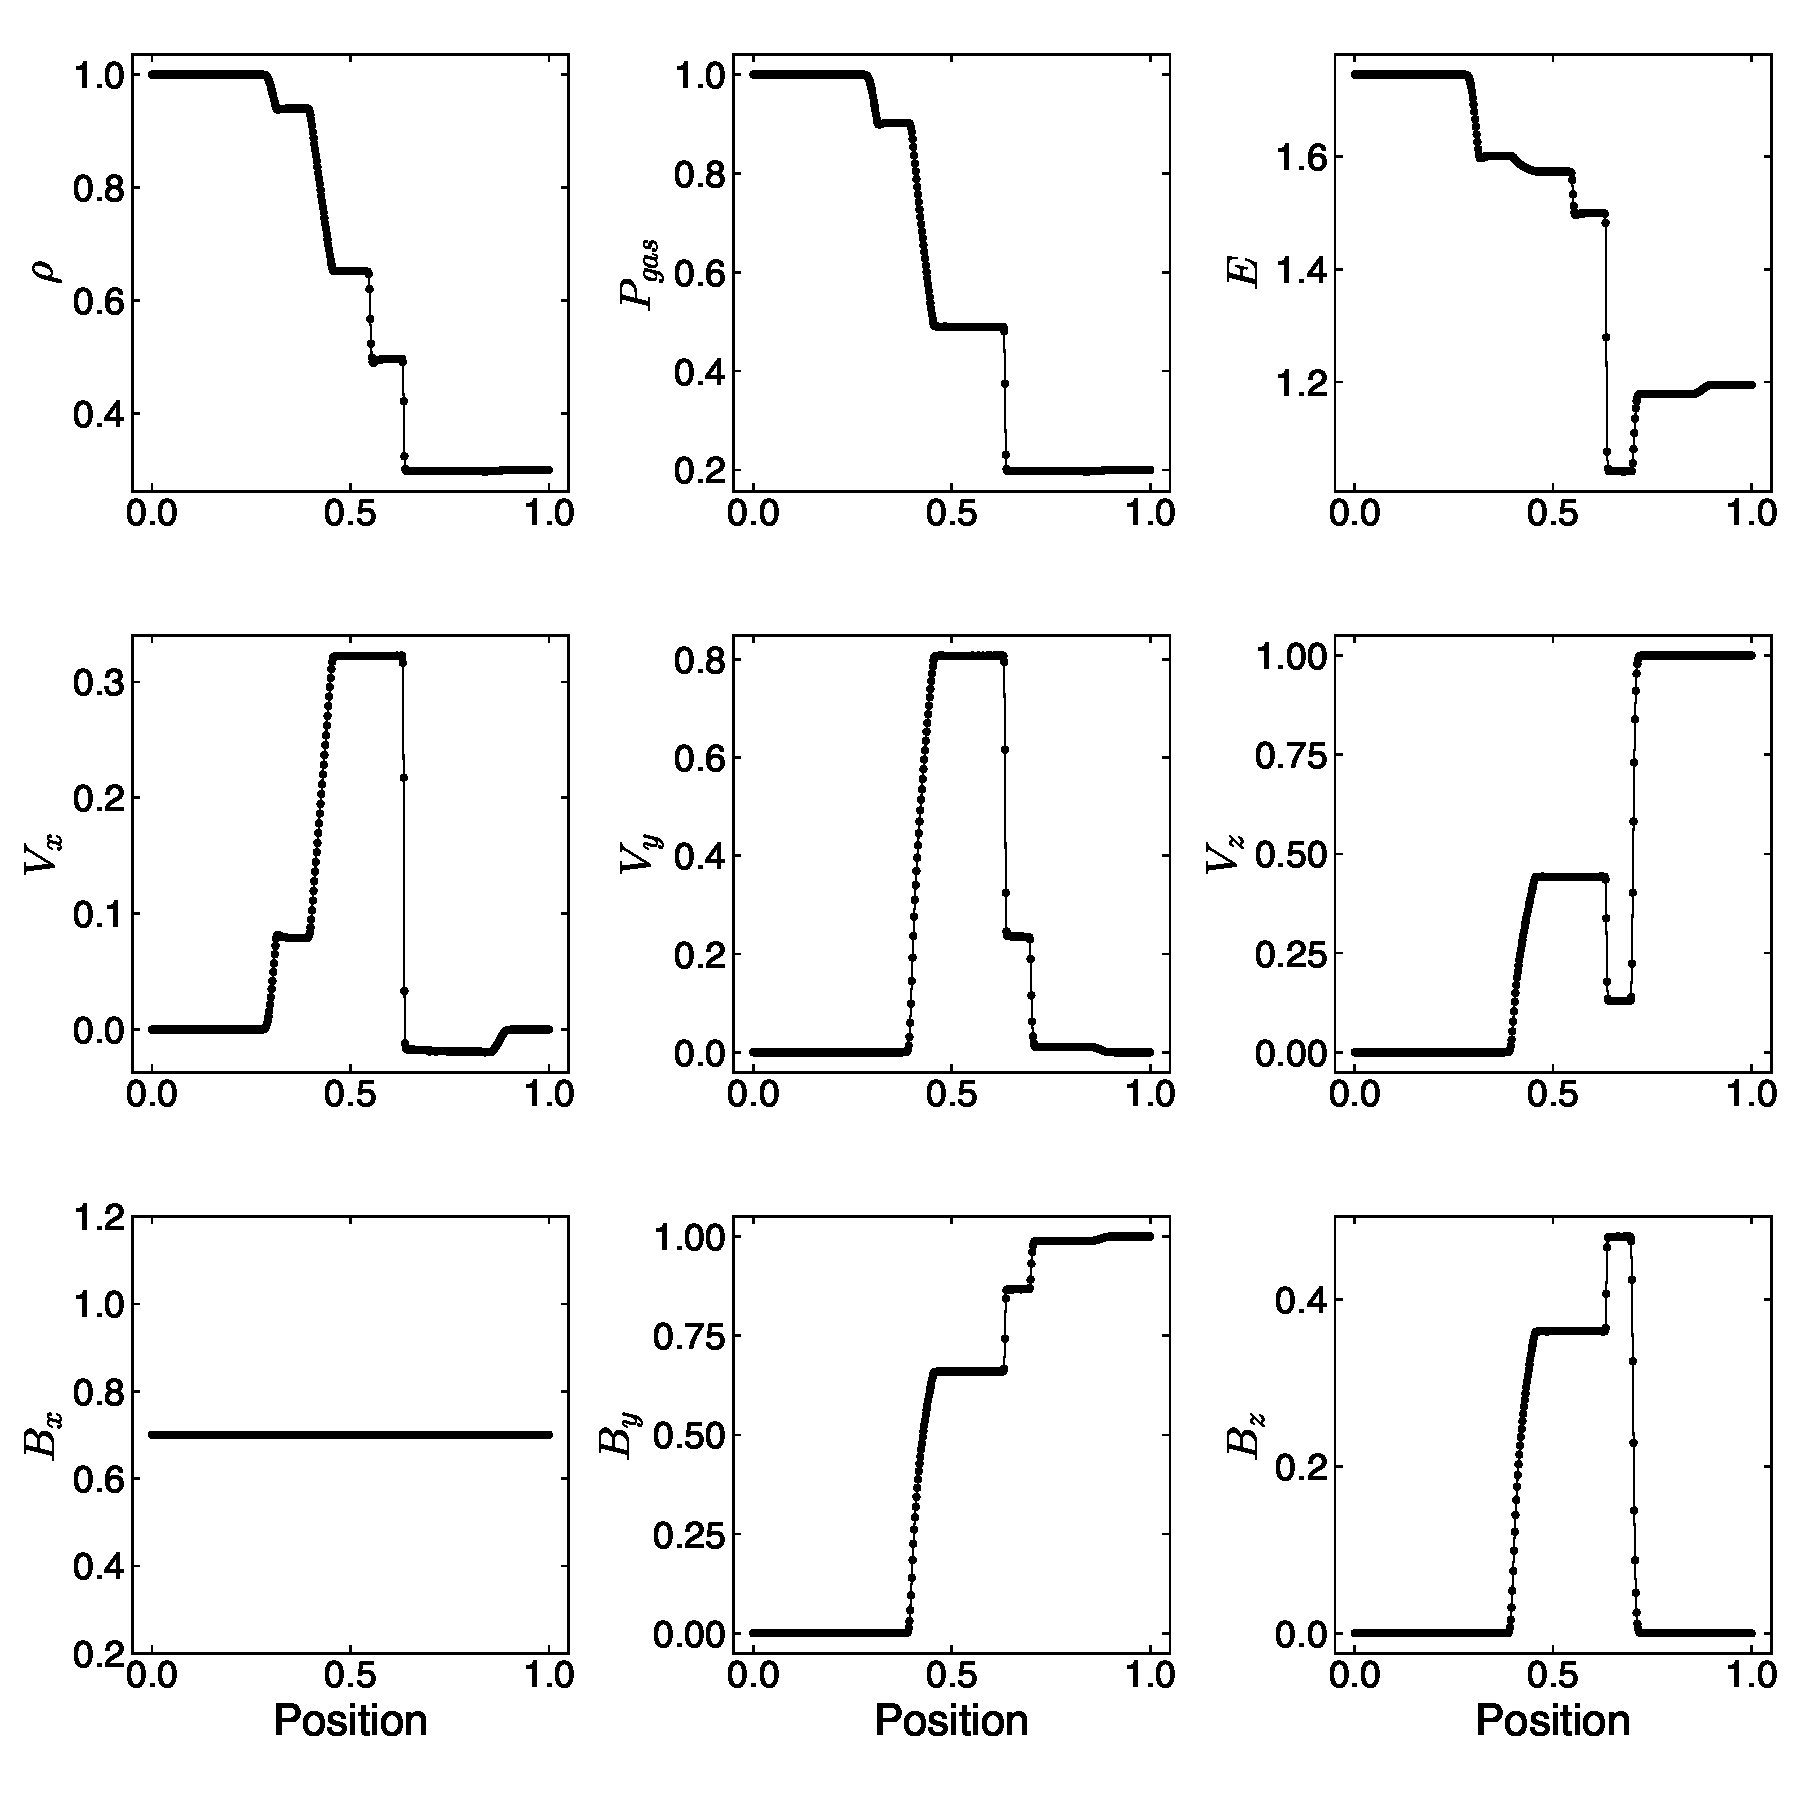
\includegraphics[width=\linewidth]{rj4d.pdf}
    \caption{Ryu \& Jones 4d Shock Tube solution \citep{ryu_jones_1995}.
    \href{https://github.com/bcaddy/caddy-et-al-2023/blob/4c9c5ef905902e54e50943d0a261bd5b08342225/python/shock-tubes.py}{\img{../latex-src/github.png}}}
    \label{fig:rj-4d}
\end{figure}

\paragraph{MHD Einfeldt Strong Rarefaction}

The MHD Einfeldt Strong Rarefaction test \citep{einfeldt_1991} creates a strong outflow and central vacuum state. The diverging solution leads to an extremely strong and fast rarefaction where the energy is dominated by kinetic energy and as such can often reveal challenges for finite-volume methods with near-vacuum states, since some Riemann solvers will return unphysical solutions with negative density or negative internal energy. High values of the outflow velocity ($V_{out}\ge3$) can also lead to spurious oscillations in the solution. $V_{out} = 2$ was chosen for this test \citep{charm_2011}. Cholla performs well on this test with no spurious oscillations or unphysical negative values.

\begin{figure}[ht!]
    % \epsscale{0.5}
    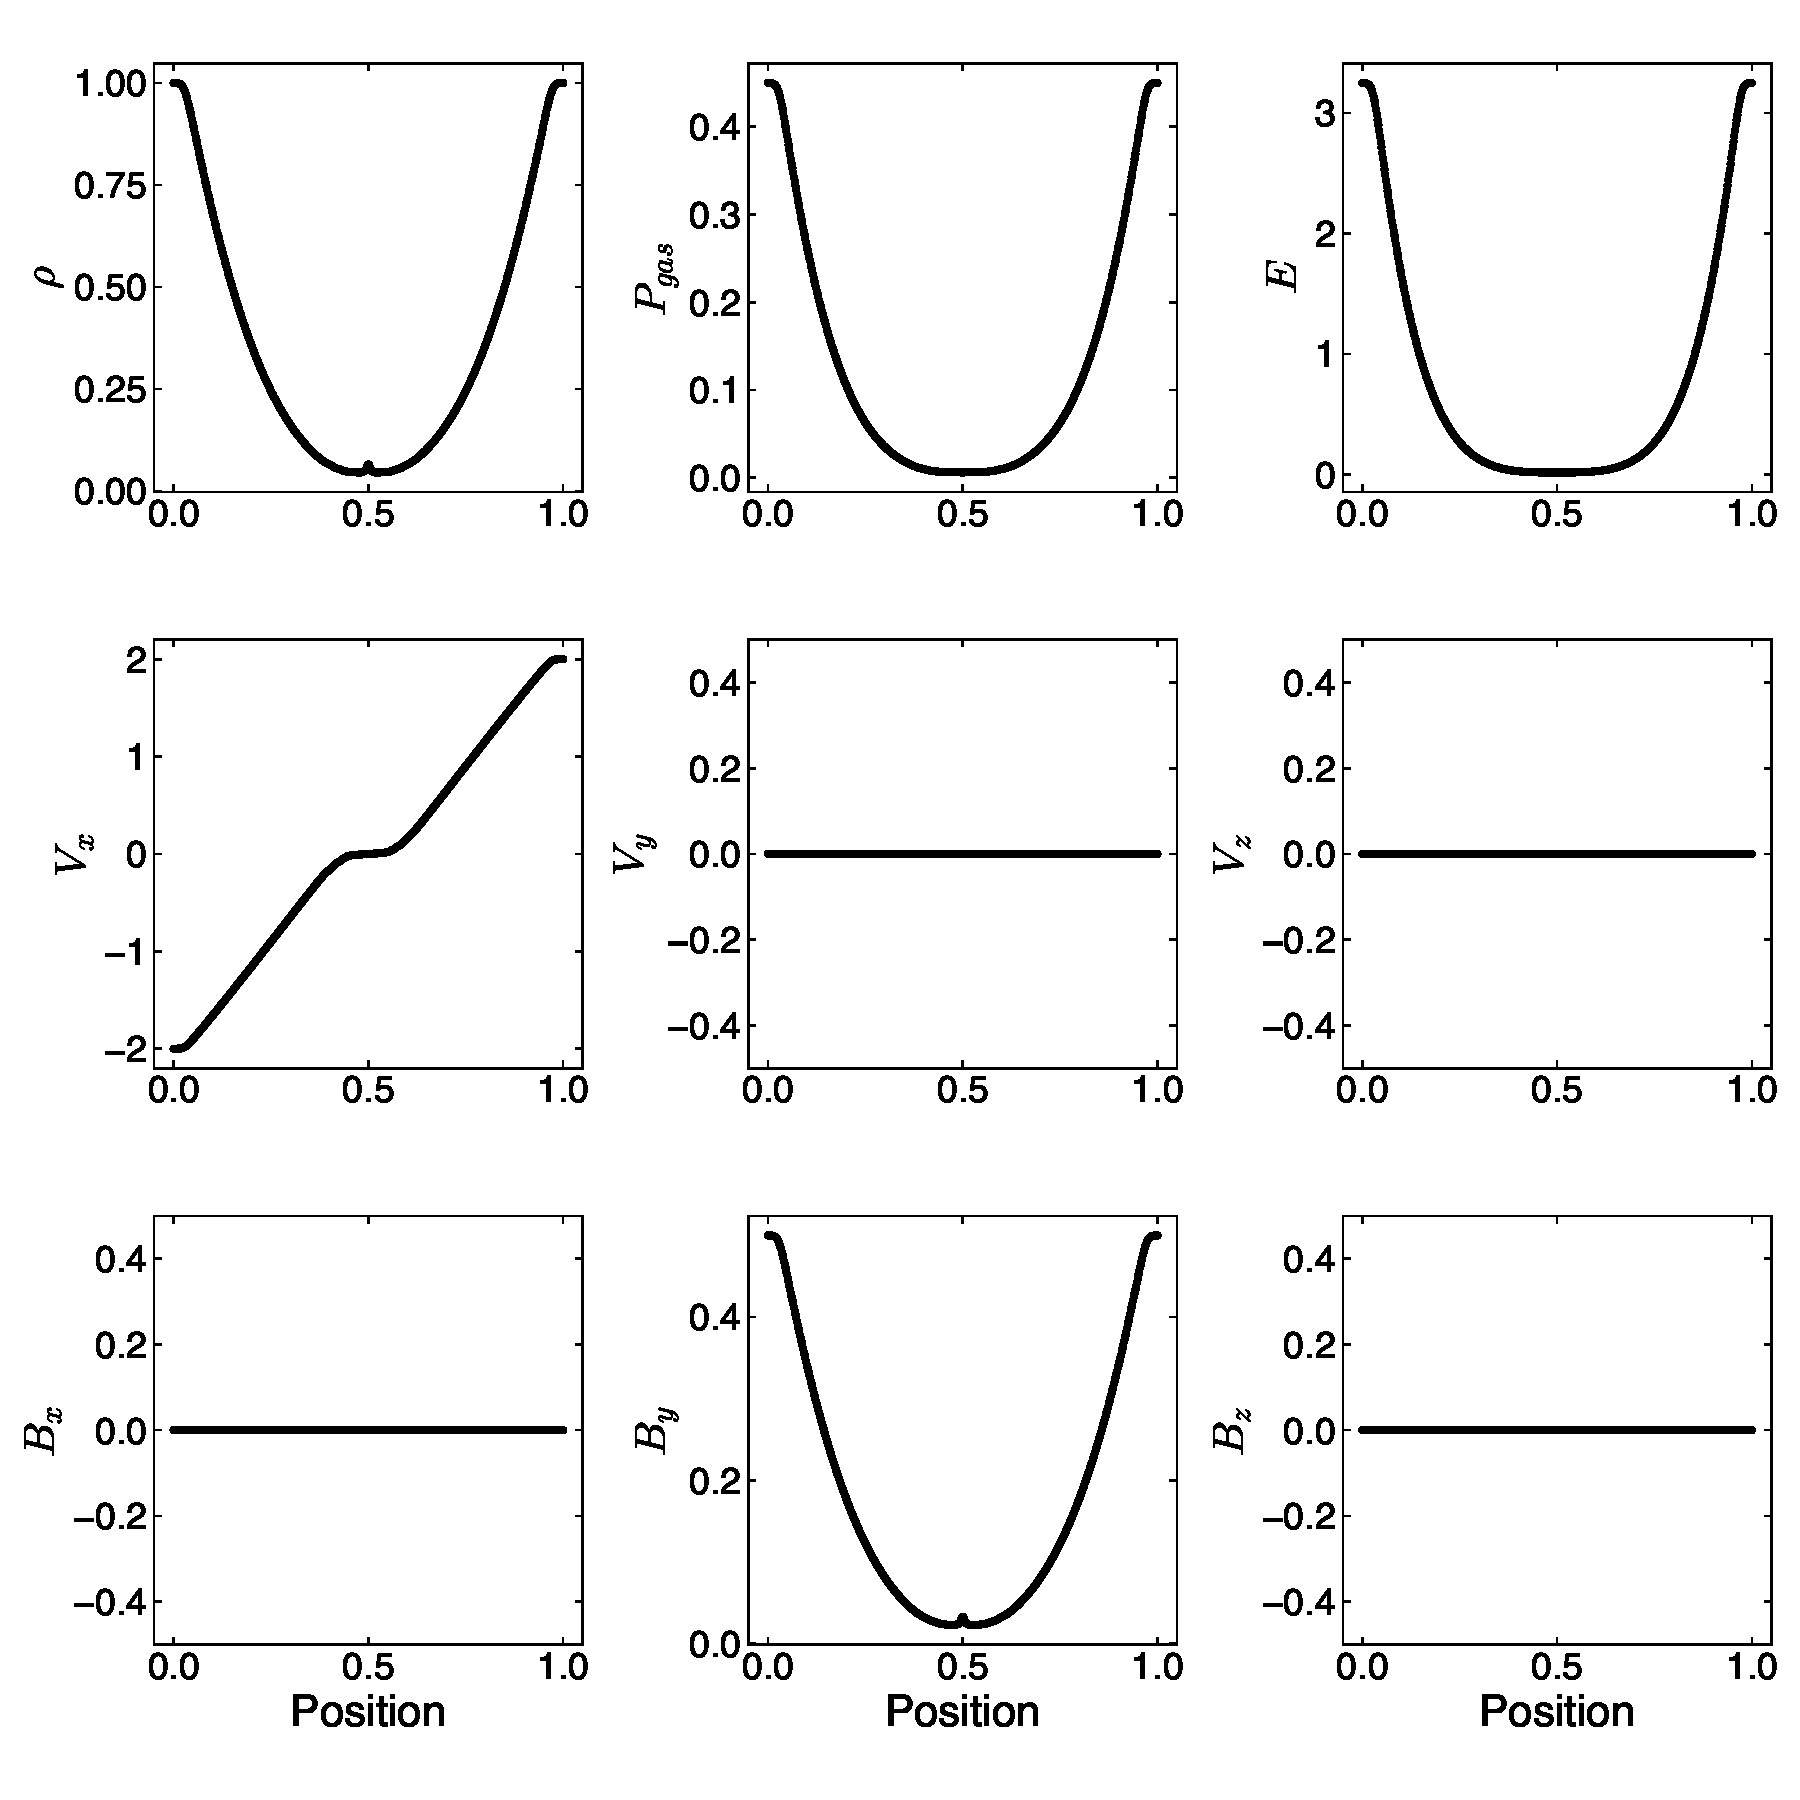
\includegraphics[width=\linewidth]{einfeldt.pdf}
    \caption{MHD Einfeldt Strong Rarefaction solution \citep{einfeldt_1991}.
    \href{https://github.com/bcaddy/caddy-et-al-2023/blob/4c9c5ef905902e54e50943d0a261bd5b08342225/python/shock-tubes.py}{\img{../latex-src/github.png}}}
    \label{fig:einfeldt}
\end{figure}

\subsubsection{MHD Blast Wave in a Strongly Magnetized Medium}
\label{sec:mhd-blast}

Blast waves in different forms are excellent tests for hydrodynamics and MHD codes. They combine strong shocked flows, smooth flows, and, in MHD, strong magnetic fields. The results are qualitative rather than quantitative, but thoroughly test the robustness of the algorithm and are excellent regression tests for automated testing (see Section \ref{sec:testing}). For this test we use $\beta = 0.2$; like \cite{stone_2009}, we find instabilities if $\beta$ is decreased by a factor of 10.

The background state is
$\rho = 1.0$,
$P = 0.1$,
$v_x = 0.0$,
$v_y = 0.0$,
$v_z = 0.0$,
$B_x = 1/\sqrt{2}$,
$B_y = 1/\sqrt{2}$,
$B_z = 0.0$,
and the over pressure region is a central sphere of size $R = 0.1$ which has $P=10.0$. The test is then run on a domain of $1\times1.5\times1$ with a resolution of $200\times300\times200$ cells until $t = 0.2$. Figure \ref{fig:blast} shows contours of the density and magnetic energy fields in an $x-y$ slice through the center of the domain. The contours are smooth and symmetric and show clear elongation of the blast wave rarefaction parallel to the magnetic field. The blast wave propagates slowly parallel to the magnetic field but much more rapidly perpendicular to the magnetic field.

\begin{figure}[ht!]
    % \epsscale{0.5}
    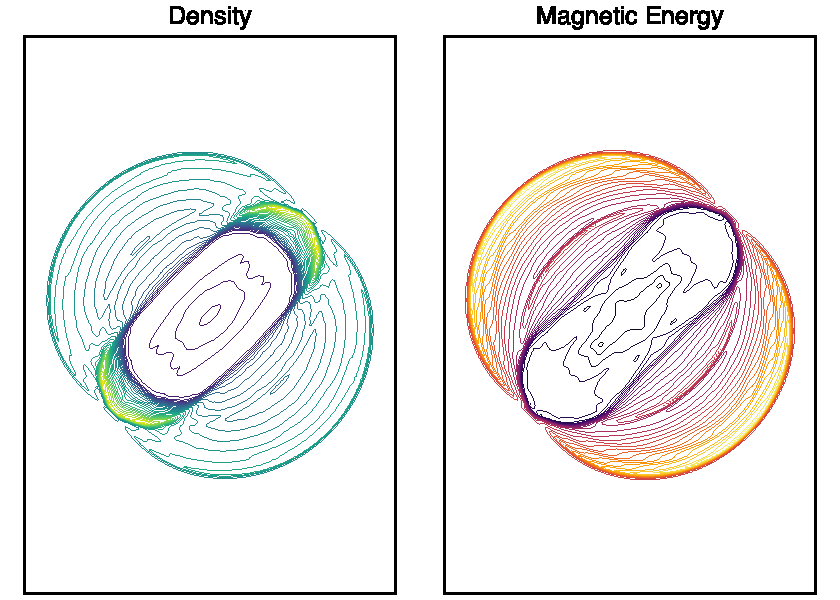
\includegraphics[width=\linewidth]{mhd-blast.pdf}
    \caption{Contour plot of the MHD blast wave test at $t=0.2$. 30 evenly spaced contours are shown in an $x-y$ slice through the center of the domain. \href{https://github.com/bcaddy/caddy-et-al-2023/blob/8f5051180971c6d63423db42e05c3d1fa1ec9785/python/blast-wave.py}{\img{../latex-src/github.png}}}
    \label{fig:blast}
\end{figure}

\subsubsection{Orszag-Tang Vortex}
\label{sec:otv}

The Orszag-Tang vortex is a standard 2D MHD test from \cite{otv_1979}. While it does not provide a quantitative measure of accuracy like the linear wave tests or a test of the robustness of the method like the MHD blast wave, it does have a very complex flow that is sensitive to changes in the integrator, making it ideal for regression testing.

The test was conducted on a periodic domain of $1\times1\times1$ with a resolution of $192\times192\times192$ cells until $t = 0.5$ with the following initial conditions:
$\rho = 25 / \left( 36 \pi \right)$,
$P    =  5 / \left( 12 \pi \right)$,
$v_x  = \sin 2\pi y$,
$v_y  = -\sin 2\pi x$,
$v_z  = 0.0$,
$A_x  = 0.0$,
$A_y  = 0.0$,
$A_z  = \left( B_0/4\pi \right) \left( \cos{4\pi x} + 2 \cos{2\pi y} \right)$, with $B_0 = 1\sqrt{4\pi}$.
The results, plotted in Figure \ref{fig:otv}, can be compared directly to Figure 22 in \cite{stone_athena_2008} as a qualitative check for correctness of the flow structure.

\begin{figure}[!ht]
    % \epsscale{0.5}
    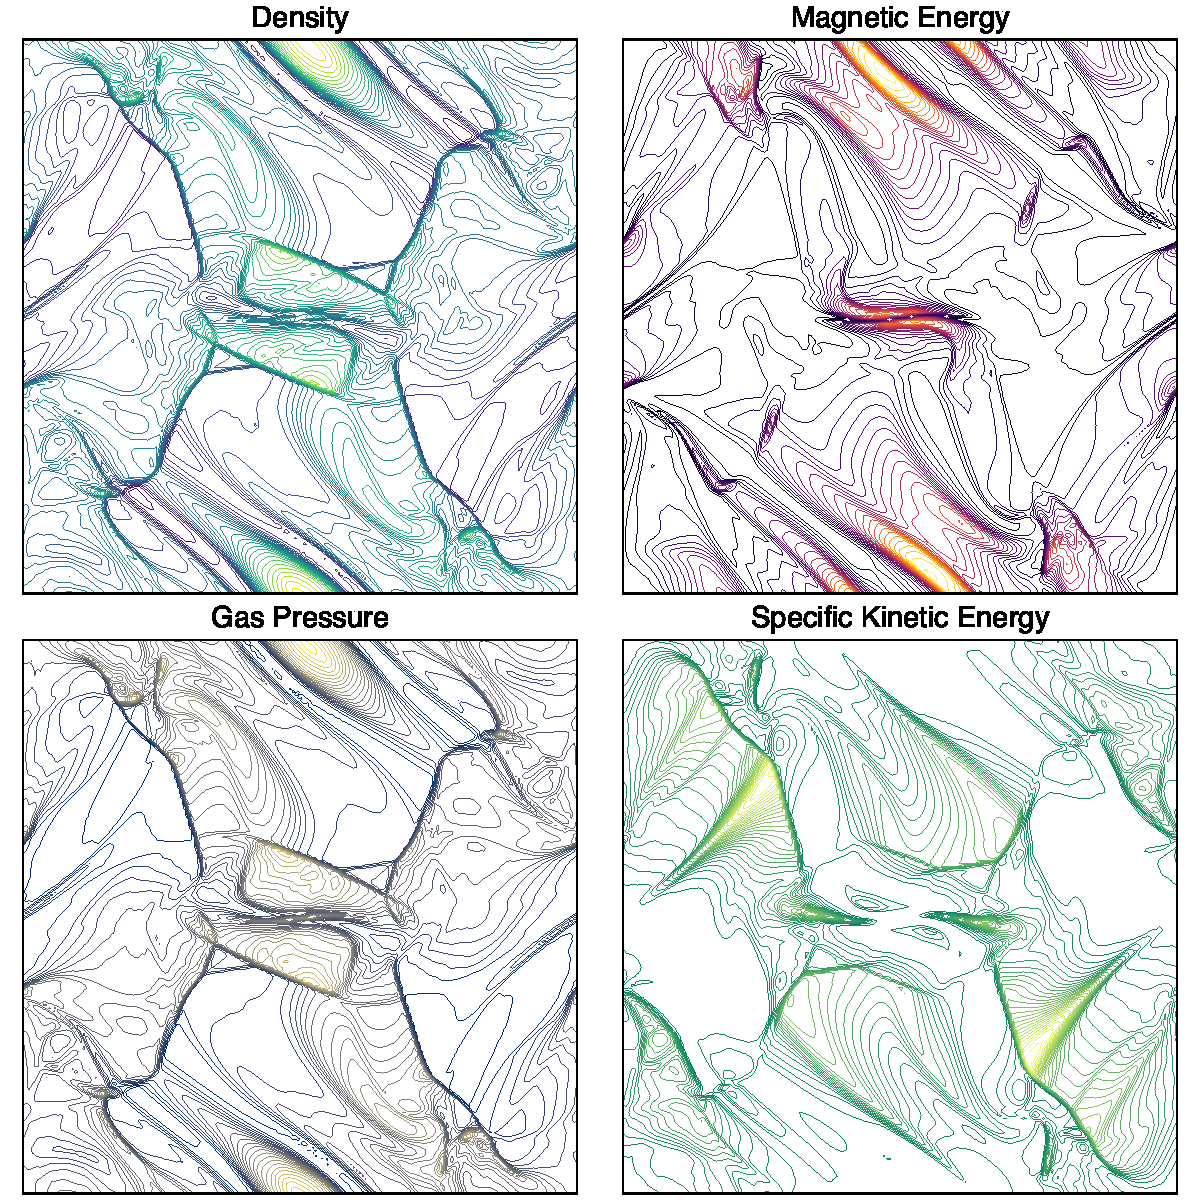
\includegraphics[width=\linewidth]{orszag-tang-vortex.pdf}
    \caption{Contour plot of the Orszag-Tang Vortex at $t=0.5$. Thirty evenly spaced contours are shown for each plot in an $x-y$ slice through the center of the domain.  \href{https://github.com/bcaddy/caddy-et-al-2023/blob/8f5051180971c6d63423db42e05c3d1fa1ec9785/python/orszag-tang-vortex.py}{\img{../latex-src/github.png}}}
    \label{fig:otv}
\end{figure}

\subsection{MHD Performance Tests}
\label{sec:mhd-perf-tests}

Given that Cholla is a massively parallel code, its scaling properties warrant discussion. We focus on weak scaling rather than strong scaling as our primary goal, since good weak scaling enables much larger problems to be simulated, while strong scaling rapidly reduces the number of cells per GPU to the point where the whole GPU cannot be utilized. Thus, GPUs may not be a good choice for algorithms and applications that require strong scaling. Results of our weak scaling tests are shown in Figure \ref{fig:scaling-weak-efficiency}.

All of the weak scaling tests shown were performed with a slow magnetosonic wave perturbation (described in Section \ref{sec:lwc}), periodic boundary conditions, in double precision, and with $459^3$ cells per MPI rank; each rank is assigned one GPU. We employ the second order piecewise linear reconstruction method with limiting in the characteristic variables. The wave is evolved for 100 time steps and the resulting time per step is averaged over the total number of time steps, excluding setup and tear down time. The slow wave was chosen due to the fact that the HLLD Riemann solver does not resolve it and as such it is difficult to accurately advect. This problem requires that every cell be updated in each time step, and should thus provide a reasonable estimate for a typical full-grid update in a simulation.

Our primary scaling tests were performed on the \textit{Frontier} Supercomputer at the Oak Ridge Leadership Computing Facility. \textit{Frontier} utilizes AMD Radeon Instinct MI250X GPUs, each of which contains two Graphics Compute Dies (GCDs) that largely function as separate GPUs and can be treated as such in software. Thus, for the sake of clear comparison to other systems, we will refer to each GCD as a single GPU for the remainder of this paper.

On \textit{Frontier} Cholla updates $2.04\times10^8$ cells per second per GPU when running with a single GPU. On 74,088 GPUs, nearly the entirety of \textit{Frontier}, Cholla performs $1.67\times10^8$ cell updates per second per GPU, with a weak scaling efficiency of 82.2\%. The 74,088 GPU run updated a total of $1.24\times10^{13}$ cells per second on a total grid size of $19,278^3$ cells.

With a single MPI rank there is no communication overhead, as no halo cells need to be exchanged. As the number of ranks grows the MPI overhead quickly stabilizes at around 15ms with a moderate increase when running on the full size of \textit{Frontier}. Perhaps most importantly, the VL+CT integrator scales almost perfectly and takes up most of the time on each time step, dominating over the MPI communication time by nearly a factor of 10. Overall these tests demonstrate that Cholla has excellent weak scaling up to the full size of \textit{Frontier}.

% Performance on different hardware: CRC V100+PPC, CRC A100+x86, Summit, Frontier, Grace Hopper?

\begin{figure}[ht!]
    \epsscale{0.5}
    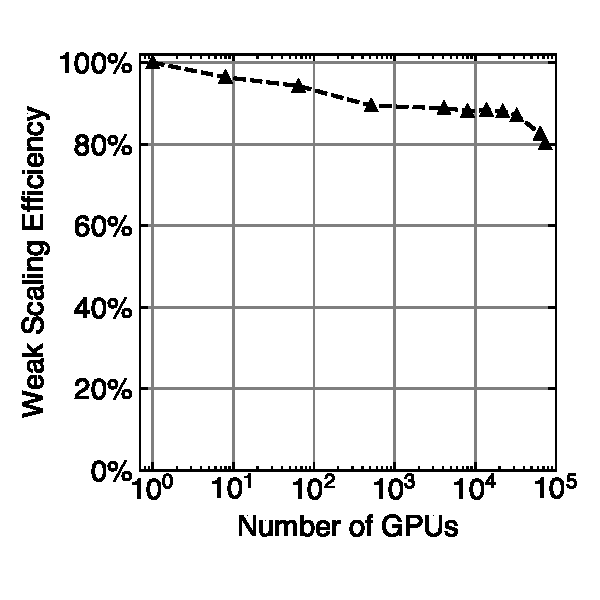
\includegraphics[width=0.5\linewidth]{scaling_tests_weak_efficiency.pdf}
    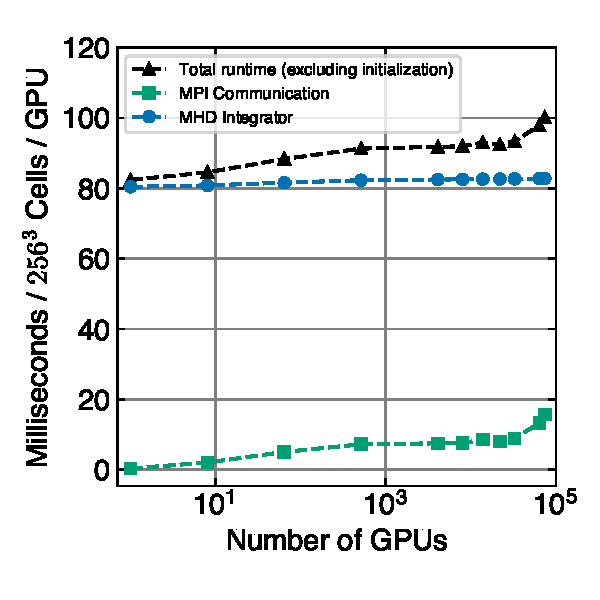
\includegraphics[width=0.5\linewidth]{scaling_tests_ms_per_gpu.pdf}
    \caption{Weak scaling performance of Cholla MHD. When running on a single GPU Cholla updates $2.04\times10^8$ cells per second per GPU; the largest run with 74,088 GPUs updates $1.67\times10^8$ cells per second per GPU, a weak scaling efficiency of 82.2\%. The 74,088 GPU run updates a total of $1.24\times10^{13}$ cells per second. \href{https://github.com/bcaddy/caddy-et-al-2023/blob/4612068c56b05fbb3286bb96228c65862a6e3c10/python/scaling_plots.py}{\img{../latex-src/github.png}}}
    \label{fig:scaling-weak-efficiency}
\end{figure}
